
\section{Exploration Outlook}

In all, 2.2 km of new cave was found during the 2010 Vodna Sled
expedition, taking \passage{Vrtnarija} to 8.776 km.

We are in the extremely fortuitous circumstance where we finish the year
with considerably more leads in the \passage{Migovec} cave systems than we started
with. The \passage{Vrtnarija} camp was derigged with the certainty that we
will be back next year camping in the same location. Gas cylinders and
cans of fish were left sealed in Daren drums with a rock of carbide to
keep them dry, the carry mats and tents were left standing to air, and
we have a considerable armoury of rope brought back from the pushing
fronts waiting for the 2011 team.

\tweet{3:21PM Aug 15th, 2010}{Van returned, all safe and sound, gear unpacked into the familiar dusty cramped confines of stores. Plans already fermenting for 2011! Out.}

The work by the JSPDT in the Autumn has `opened up' \passage{M2} once again
and brought the possibility of forging a connection back to the table.

The pushing of the \passage{Republica} streamway (now \passage{Insomnia}) to within a
few metres of the maximum depth of the cave has reawakened the
possibility of further depth extension to \passage{Vrtnarija}. Expedition
members have mooted the possibility of establishing an additional 2-man
`deep camp' to benefit pushing trips in the lower reaches of the cave,
particularly any revisits to the far North end of the system.


\section{Migovec's Long Term Prospects}


\begin{marginfigure}
\checkoddpage \ifoddpage \forcerectofloat \else \forceversofloat \fi
\centering
 \frame{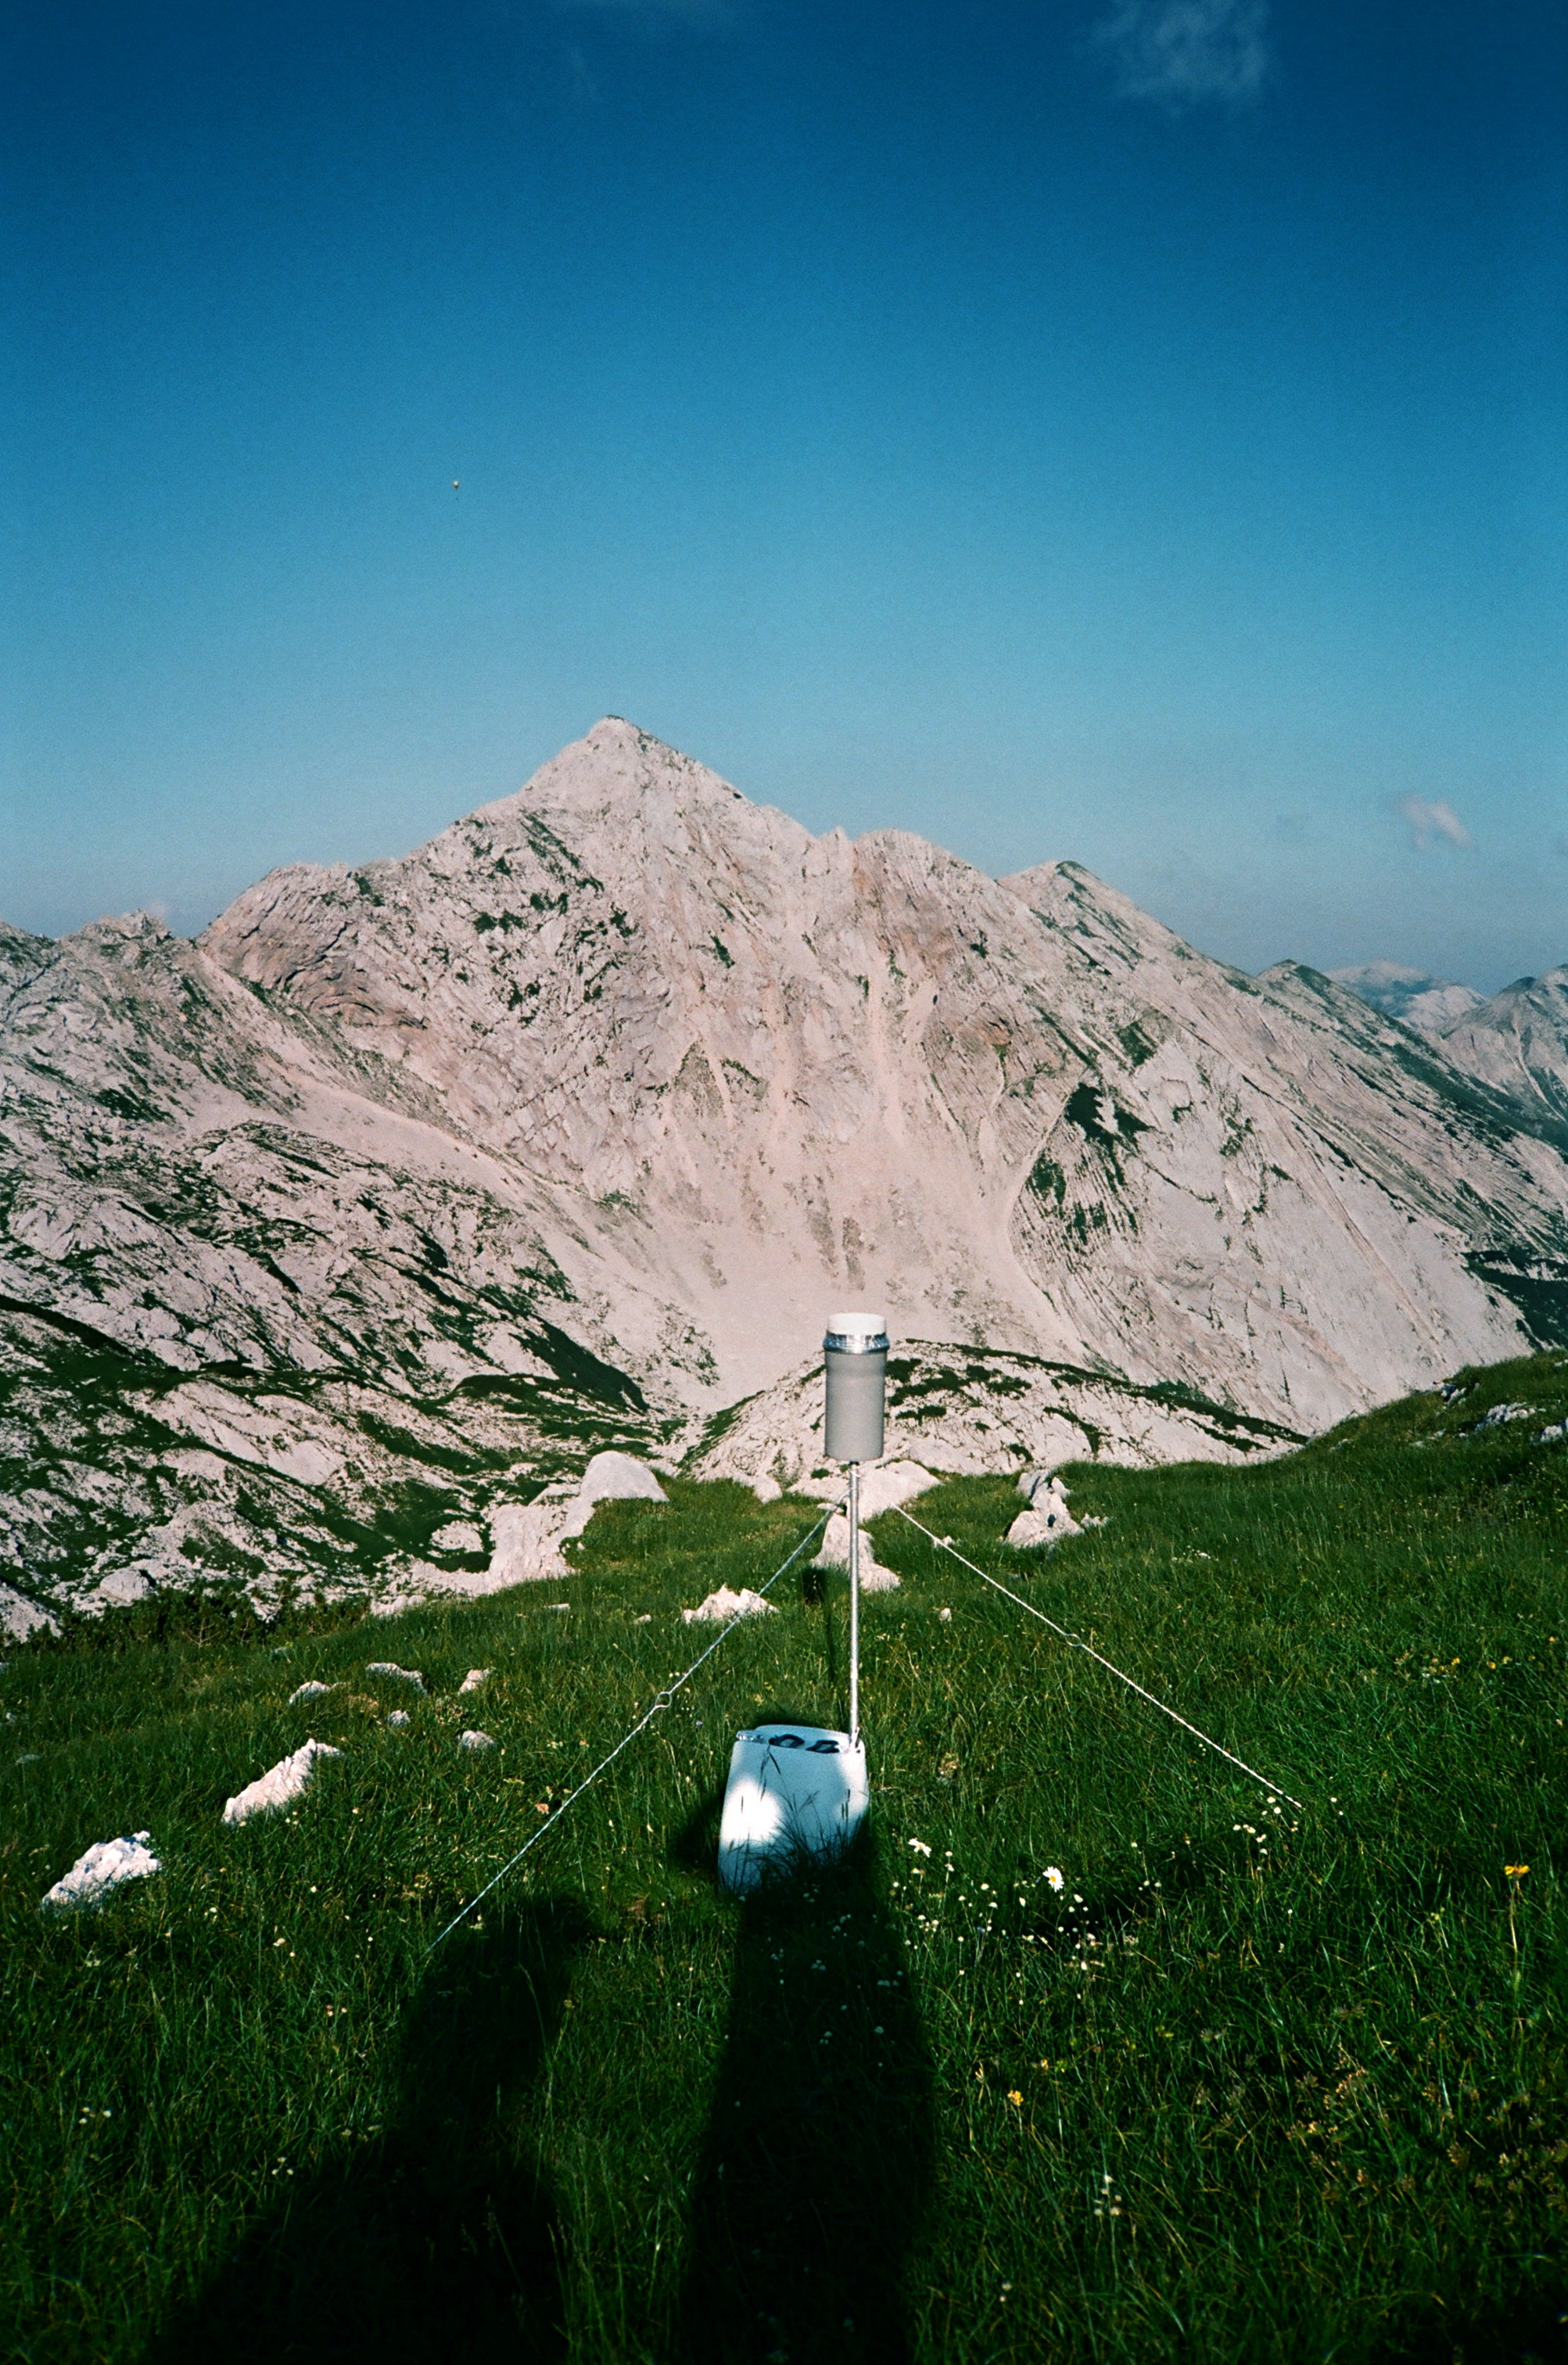
\includegraphics[width=\linewidth]{2010/outlook/jarvist frost - olympus xa - superia 100 - 2009 - rain gauge with skrbina in background--orig.jpg}} 
 \caption{A rain gauge with an enviable view of \passage[mountain]{Migovec} and its neighbouring mountain \passage[mountain]{Škrbina}. \pic{Jarvist Frost}}
 \label{rain gauge}
\end{marginfigure}

It has been a recurrent discussion in our club as to when we will run
out of new cave to discover in \passage[mountain]{Migovec}. Almost all of our fruitful
exploration has taken place within a single square kilometre of the flat
topped mountain.

\passage[mountain]{Migovec}, being part of a mountain chain that is the first high altitude
interruption to moist air from the Adriatic, receives an extremely
significant level of rainfall. This summer, Jaka Ortar, a Slovenian
geographer, recorded 210 cm of rain on \passage[mountain]{Migovec} in 100 days (28\(^{th}\)
July-3\(^{rd}\) November) with his network of rain gauges. However we
have never found any large rivers underground --- the known cave can
only account for a tiny percentage of the total drainage for the
plateau.

Our current hypothesis is that there is no \textit{master system}
gathering the water, but instead a complex hydrology induced by cave
passage intersecting the underlying (as yet, unvisited) band of
Cretaceous shales.

For all \passage{Vrtnarija}'s complexity, the entire cave can be fitted
into a slab of limestone slanted at 66 degrees and just
\(1000\times150\times1000\) m.

Certainly, as long as we can continue to find entrances through the
frost shattered and heavily cratered surface, there will be enough cave
in \passage[mountain]{Migovec} for decades more of exploration.
